\documentclass[../main.tex]{subfiles}

\begin{document}
Im Gegensatz zu General Purpose CPUs lassen sich mithilfe von Coprozessoren deutlich höhere Parallelisierungsgrade erzielen. Gegenüber GPUs haben sie den Vorteil, dass die Kerne eines Coprozessors einen größeren Befehlssatz verfügen, mit dem sie nicht nur Befehlssequenzen, sondern auch bedingte Sprünge ausführen können. Mit GPUs lässt sich dagegen eine weitaus höhere Parallelität erreichen. Mit der Max Pooling-Operation ist die Fähigkeit von Coprozessoren, auch Code mit Verzweigungen parallel auszuführen, von Nutzen. 
In dieser Arbeit soll auch eine Implementierung des CNNs erstellt werden, die Berechnungen an Coprozessoren. Ein direkter Vergleich dieser Implementierung mit Tensorflow hat nur bedingte Aussagekraft, da Tensorflow laut der offiziellen Dokumentation nur für den Einsatz auf CPUs, GPUs und TPUs optimiert ist. Coprozessoren werden von Tensorflow dagegen nicht explizit unterstützt. (vgl. \cite{aboutTensorflow}) Ein Vergleich zwischen dieser Implementierung und den anderen beiden in dieser Arbeit behandelten optimierten Implementierungen lässt allerdings Rückschlüsse darauf ziehen, wie der Performancegewinn unter Zuhilfenahme eines Coprozessors einzuordnen ist. 

Die DHBW Stuttgart besitzt einen Server, der mit einer General Purpose CPU(Intel Xeon E5-2650L) und zwei Coprozessoren(Intel Xeon Phi) ausgestattet ist. Beim Xeon Phi handelt es sich um eine PCIe-Erweiterungskarte, auf der eine spezielle CPU mit 60 Kernen und einer Taktrate von 1\,GHz, sowie ein DDR5-Arbeitsspeicher mit einer Größe von 8\,GB verbaut sind. Für diese Arbeit wurde den Studenten freundlicherweise ein SSH-Zugang zur Verfügung gestellt. Die in diesem Kapitel betrachtete Implementierung soll auf dem genannten Server getestet und dementsprechend auch für dessen Prozessoren optimiert werden. 
\section{Intel Xeon Phi Coprozessor}
Beim Intel Xeon Phi handelt es sich um einen Coprozessor, der in Form einer PCIe-Erweiterungskarte (siehe Abbildung \ref{pic:xeonphicard}) mit dem Hostsystem verbunden werden kann und numerische Operationen durch Parallelisierung über bis zu 72 Rechenkerne, sowie durch Vektorisierung unterstützt. Zusätzlich zum Prozessor selbst ist auf der Erweiterungskarte ein DDR5-Arbeitsspeicher verbaut. Bei Bedarf kann der Xeon Phi ein eigenes Betriebssystem ausführen und damit Programme komplett unabhängig vom Hostsystem abarbeiten. (vgl. \cite{intelxeonphiprocessors})
\begin{figure}
    \centering 
       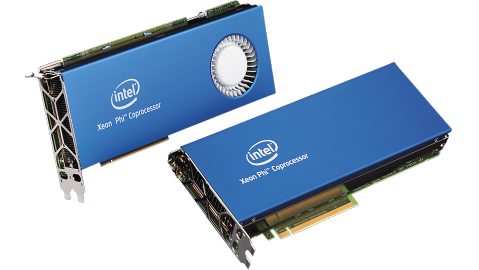
\includegraphics[width=0.5\textwidth]{../images/Schmidt/xeon_phi_cards.png} 
    \caption {Eine Erweiterungskarte mit einem Intel Xeon Phi (Quelle: \parencite{intelMICarchitecture})} 
    \label{pic:xeonphicard} 
\end{figure} 
\subsection{Geschichte}
%TODO
\subsection{MIC-Archtektur}
Der Xeon Phi basiert auf der von Intel entwickelten MIC-Architektur. MIC steht dabei für "Many Integrated Cores". 
Wie in Abbildung \ref{pic:knightscorner} am Beispiel der Mikroarchitektur Knigths Corner zu sehen ist, kommunizieren die Kerne, der Arbeitsspeicher und die PCIe-Schnittstelle untereinander über einen Ringförmigen Datenbus mit einer Busbreite von 64 Bytes. (vgl. \cite{xeonphiJumpstart})
\begin{figure}
    \centering 
       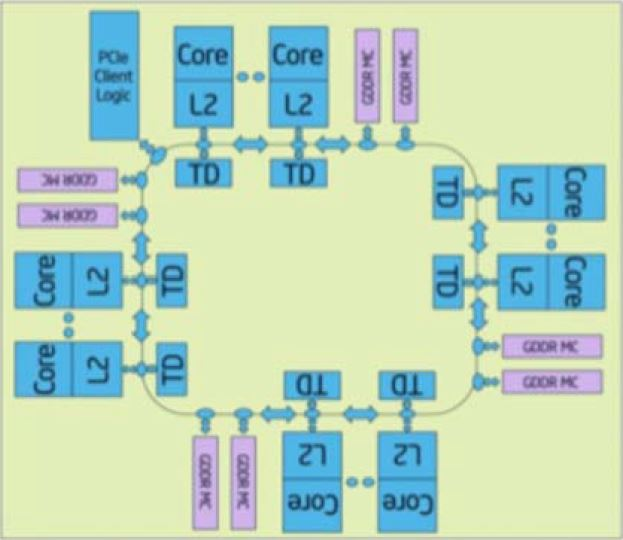
\includegraphics[width=0.5\textwidth]{../images/Schmidt/intel_mic_diagram.jpg} 
    \caption {Mikroarchitektur Knights Corner (Quelle: \parencite{xeonphiJumpstart})}
    \label{pic:knightscorner} 
\end{figure}
Zur Verminderung der Verlustleistung und der damit verbundenen Abwärme takten die einzelnen Rechenkerne langsamer als vergleichbare General Purpose CPUs. Der hohe Durchsatz des Coprozessors kann erreicht werden, weil Operationen auf viele Kerne verteilt und Operanden mithilfe der breiten Speicheranbindung zeitnah abgerufen werden können. (vgl. \cite{xeonphiJumpstart})
\subsection{Anbindung an das Hostsystem}
Mit dem Hostsystem ist der Xeon Phi über PCIe x16 verbunden. Dieser Bus lässt eine Bandbreite von 8\,GB/s zu. Verglichen mit der Bandbreite der Speicheranbindung des Hostsystems, sowie des Datenbusses innerhalb des Xeon Phi ist diese Bandbreite sehr gering. Abbildung \ref{pic:xeonphiBandwidths} vermittelt einen Eindruck über die Busbreiten innerhalb eines Systems mit zwei Prozessoren, DDR3-Arbeitsspeichern, und einem Rechenbeschleuniger bestehend aus einem Intel Xeon Phi und DDR5-Speicher. (vgl. \cite{interDeviceCommunication})
\begin{figure}
    \centering 
       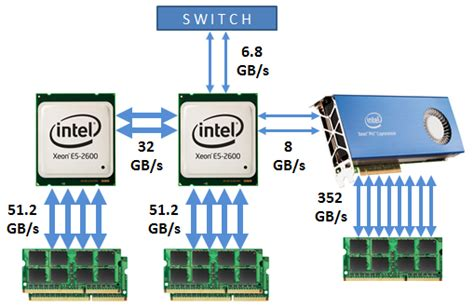
\includegraphics[width=0.5\textwidth]{../images/Schmidt/xeonphi_bandwidths.jpg} 
    \caption {Busbandbreiten eines Systems mit DDR3-Arbeitsspeicher und Intel Xeon Phi (Quelle: \parencite{interDeviceCommunication})}
    \label{pic:xeonphiBandwidths} 
\end{figure}
In Anwendungen, bei denen Daten zwischen dem Hostsystem und dem Xeon Phi geteilt werden müssen, ist die Übertragung dieser Daten eine kritischer Engpass. Der Aufwand zur Kommunikation zwischen den beiden Systemen hat großen Einfluss auf die Performance des Gesamtsystems. Der Programmierer hat dafür Sorge zu tragen, dass der Datenaustausch zwischen dem Host und dem Rechenbeschleuniger möglichst effizient verläuft. Die Beachtung folgender Faustregeln trägt zu einer hohen Effizienz des Offloads bei: 
\begin{itemize}
\item Daten zum Coprozessor transferieren und dort behalten (vgl. \cite{xeonphiJumpstart})
\item Möglichst große Rechenoperationen auslagern (vgl. \cite{xeonphiJumpstart})
\item Auf dem Coprozessor bereits existierende Daten wiederverwerten (vgl. \cite{xeonphiJumpstart})
\end{itemize}
\section{Nutzungsmodelle}
Zur Planung einer Software, die einen Xeon Phi benutzen soll, gehört die Überlegung, welche Operationen sich zur Ausführung auf dem Coprozessor eignen und welche Rechenschritte auf dem Hostsystem ausgeführt werden sollten. Abhängig von dieser Verteilung sollte bestimmt werden, auf welche Weise der Coprozessor verwendet werden soll. Es kann zwischen mehreren Nutzungsmodellen gewählt werden, die bekanntesten davon werden nachfolgend vorgestellt. 
\subsection{Automatic Offload}
Das für den Programmierer einfachste Nutzungsmodell ist Automatic Offload. Bei diesem Modell entscheidet das Programm zur Laufzeit, ob numerische Berechnungen auf dem Coprozessor oder dem Hostsystem ausgeführt werden sollen. Der Programmierer muss dazu keine Vorkehrungen im Quellcode treffen. Die dazu notwendige Entscheidungslogik ist bereits in einigen vorkompilierten Bibliotheken, wie der Math Kernel Library von Intel enthalten. Das bedeutet, dass sich der Programmierer bei der Nutzung von Funktionen dieser Bibliotheken keine Gedanken darüber machen muss, wann eine Auslagerung an den Coprozessor sinnvoll ist oder wie diese veranlasst wird. Ein Nachteil dieses Modells besteht allerdings darin, dass es sich nur auf dafür geeignete Bibliotheksfunktionen anwenden lässt. Zur Auslagerung von eigenem Anwendungscode lässt sich dieses Modell nicht anwenden. 
\subsection{Compiler-Assisted Offload}
Für den Fall, dass aufwändige Abschnitte des Anwendungscodes auf den Coprozessor ausgelagert werden sollen, kann dies dem Compiler explizit mitgeteilt werden. In C/C++ lässt sich dies mithilfe des Pragmas \lstinline|\#pragma offload| bewerkstelligen. (vgl. \cite{xeonphiQuickstart}) Das nachfolgende Codebeispiel soll verdeutlichen, wie dieses Pragma anzuwenden ist. 
\begin{lstlisting}[language=c, caption={Beispiel für eine Funktion, die ausgelagert werden soll (Quelle: \parencite{xeonphiQuickstart})} , captionpos=b, label=lst:compoffloadBefore, frame=single, linewidth=\textwidth, breaklines=true]
float reduction(float *data, int size) 
{ 
	float ret = 0.f; 
	for (int i=0; i<size; ++i) 
	{
		ret += data[i]; 
	} 
	return ret; 
}
\end{lstlisting}
\begin{lstlisting}[language=c, caption={Beispielfunktion mit pragma zur Auslagerung(Quelle: \parencite{xeonphiQuickstart})}, captionpos=b, label=lst:compoffloadAfter, frame=single, linewidth=\textwidth, breaklines=true]
float reduction(float *data, int size) 
{ 
	float ret = 0.f; 
	\#pragma offload target(mic) in(data:length(size))
	for (int i=0; i<size; ++i) 
	{
		ret += data[i]; 
	} 
	return ret; 
}
\end{lstlisting}
Wie in den obigen Beispielen zu sehen ist, genügt bereits das Hinzufügen einer Zeile zum Quellcode, um einen zusammenhängenden Codeabschnitt (in diesem Beispiel die \lstinline|for|-Schleife) an den Coprozessor auszulagern. Die Angabe \lstinline|target(mic)| legt dabei fest, dass an einen Coprozessor mit der MIC-Architectur ausgelagert werden soll. Die Angabe \lstinline|in(data:length(size))| teilt dem Compiler mit, dass das Array \lstinline|data| mit der Größe \lstinline|size| zum Coprozessor übertragen hin, aber nicht mehr zurück übertragen werden muss. Für die Variable \lstinline|ret| gibt es keine explizite Angabe, daher wird sie per Default vor der Berechnung zum Coprozessor hin und anschließend zum Hostsystem zurück übertragen. (vgl. \cite{xeonphiQuickstart})
Auch wenn dieses Pragma im Quellcode angegeben ist, gibt es keine Garantie dafür, dass der betroffene Codeabschnitt tatsächlich vom Coprozessor bearbeitet wird. Laut dem C99-Standard ist es dem Compiler überlassen, wie Pragmas in einem C-Programm zu behandeln sind. Pragmas sind sogar explizit dafür vorgesehen, compilerspezifische Features zu steuern. Wenn das Programm mit einem Compiler übersetzt wird, der nicht für den Offload auf einen Xeon Phi vorgesehen ist, dann sollte er dieses Pragma ignorieren und bestenfalls mit einer Warnung auf das unbekannte Pragma hinweisen. (vgl. \cite{gccDokuPragmas}) Selbst wenn der Compiler Offload-Code für einen Xeon-Phi erzeugt, dann muss das noch nicht zwangsläufig heißen, dass der Offload tatsächlich durchgeführt wird. Wenn der Coprozessor zur Laufzeit nicht Verfügbar ist, dann wird der auszulagernde Codeabschnitt trotzdem auf dem Hostsystem ausgeführt. (vgl. \cite{xeonphiQuickstart})
Compiler Assisted Offload ist dann hilfreich, wenn Teile des Anwendungscodes auf den Coprozessor ausgelagert werden sollen. Es liegt jedoch in der Verantwortung des Programmierers, geeignete Codeabschnitte auszuwählen und die zu übertragende Datenmenge gering zu halten. 
\subsection{Native}
Eine dritte Möglichkeit besteht darin, Anwendungen nativ auf dem Coprozessor laufen zu lassen. Dazu muss die Anwendung mit unter Angabe einiger zusätzlicher Compileroptionen gebaut werden. Die dabei erstellte Binary ist dann auf dem Hostsystem selbst nicht lauffähig. Sie lässt sich allerdings auf den Xeon Phi übertragen. Dieser verfügt über ein auf dem Linux-Kernel basierendes Betriebssystem, auf dem die erzeugte Binary ausgeführt werden kann. Bei einer nativen Programmausführung muss nur einmalig die Binary zum Xeon Phi übertragen werden. Zur Laufzeit ist dann keine Kommunikation mit dem Hostsystem notwendig. Auf diese Weise kann der Flaschenhals zwischen den beiden Systemen umgangen werden. (vgl. \cite{xeonphiQuickstart})
Es ist allerdings nicht für jede Software von Vorteil, nativ auf dem Coprozessor zu laufen. Die Performance bei der Ausführung serieller Programmabschnitte nimmt bei diesem Nutzungsmodell deutlich ab, da der Xeon Phi für diese Aufgaben nicht optimiert ist. Die Performance bei der Ausführung von parallel berechenbaren Operationen nimmt nicht signifikant zu oder ab, denn sobald notwendigen alle Instruktionen und Operanden zur Verfügung stehen, wird die eigentliche Berechnung auf die gleiche Art ausgeführt. Was tatsächlich eingespart wird, sind die Datentransfers zwischen dem Hostsystem und dem Coprozessor. Aufgrund dieser Informationen kann eingeschätzt werden, ob sich eine native Programmausführung gegenüber einer Offload-Variante lohnt: Bei seltenen Wechseln zwischen längeren seriellen und parallelen Abschnitten sollte das Programm auf dem Hostsystem ausgeführt werden und bei Bedarf Rechenoperationen an den Xeon Phi auslagern. Wenn es erforderlich ist, das Programm in viele kurze serielle und parallele Abschnitte zu unterteilen, dann nimmt die Wahrscheinlichkeit zu, dass sich die native Ausführung der gesamten Anwendung auf dem Xeon Phi lohnt. (vgl. \cite{xeonphiQuickstart})
\section{Compiler}


\section{Multithreading}

\subsection{PThread}

\subsection{OpenMP}

\subsection{OpenMPI}

\subsection{Intel Threading Blocks}



\section{Intel Math Kernel Library}

\subsection{BLAS}

\subsection{Vector Mathematical Functions}



\section{Grundlegende Überlegungen}

\subsection{Parallelisierung}

\subsection{Programmiersprache}

\subsection{Datenorganisation}

\subsection{Convolution und Pooling}

\subsection{Buildsystem}



\section{Skript zur Netzwerkbeschreibung}

\subsection{Klasseneinteilung}

\subsection{Netzwerk}

\subsection{Layertypen}

\subsection{Schnittstellen zwischen Schichten}

\subsection{Netzwerkmodell}

\subsection{Netzwerkkonfiguration}



\section{Programm zur Netzwerksimulation}

\subsection{Moduleinteilung}

\subsection{Netzwerkmodell}

\subsection{Netzwerkinitialisierung}

\subsection{Hilfsfunktionen}

\subsection{Verhaltensbeschreibung der Layer}

\subsection{Datenfluss beim Fully Connected Layer}

\subsection{Organisation der Faltungsoperation}

\subsection{Implementierung des Poolings}

\subsection{Programmfluss}



\section{Anpassung der Netzwerkkonfiguration}

\subsection{Startgewichte}

\subsection{Reduzierung der Lernrate}

\subsection{Fehlerreduktion beim Convolution Layer}


\section{Vergleich mit Tensorflow}



\end{document}